%data acquisition
\section{Data Acquisition} \label{sec:dataAcquisition}

This section will clarify the method of acquiring data in this paper/report.

For data acquisition the MYB will be used to record EMG signals from muscles in the lower forearm described in \secref{sec:anatomy}. The recordings will be made on test subjects instructed to perform six different hand gestures as introduced in the protokol, \secref{sec:protokol}. As described in \secref{sec:MYB} about the MYB, the armband has a sample rate of 200 Hz. 

%According to the Nyquist theorem, to achieve a loss-less representation of the signal the sampling frequency must be at least twice the maximum frequency of interest of the original signal \cite{Pozzo2004}. In relation to this paper a sampling frequency of at least twice the maximum of the recorded signal is not possible, since muscles of the forearm have a maximum frequency of 400-500 Hz \cite{Cram2012}. This would require a sample rate of at least 1000 Hz, which cannot be achieved due to limitations in the MYB. The effect of the low sample rate of the MYB is aliasing in the recording, causing a frequency component not originally in the EMG signal. To account for this an \textbf{anti-aliasing filter is implemented}, described further in \secref{sec:prePros} on preprocessing of the signal. Thus, data will be acquired as a sampling frequency of 200 Hz.

For acquiring data a Graphical User Interface (GUI) has been designed using MatLab. In the GUI it is possible to change settings for different types of recordings. The first type of recording are of baseline. This recording is made in order to be able to remove signal artefacts. The second recording type is Maximum Voluntary Contraction (MVC) which is a 15 second recording of the subjects maximum contraction in one gesture that can be kept constant for 15 seconds. The third type of recording is of EMG signals used in data processing. The recordings of EMG signals are based on fractions of the MVC which can be set using a slider in the GUI. As stated in the protokol, \secref{sec:proto}, three contraction levels will be used: 20\%, 40\% and 60\%. The level of contraction defines the height of the plateau of a trapezoid trajectory which will be plotted in a window in the GUI. When doing EMG recordings the subjects must perform the instructed gesture to control the height of a cursor in the trapezoid plot to best match the trajectory of the trapezoid. The subject only controls the height of the cursor as the cursor will automatically move forward along the x-axis in relation with time. The recording time is 15 seconds, with five seconds each on the trajectory incline, plateau and decline \fxnote{is this true?}. This approach provides data on a performed gesture in both the transition and steady state phase, at the specified contraction level. A screencap of the GUI is shown if \figref{fig:GUIplot} during acquisition of EMG data. 
During recordings the investigators will evaluate if the subject followed the trajectory well enough, and following the data acquisition for a subject a PCA will be used to evaluate if the acquired data are applicable. If the data is not usable a new recording will be made. 

\begin{figure}[H] 
	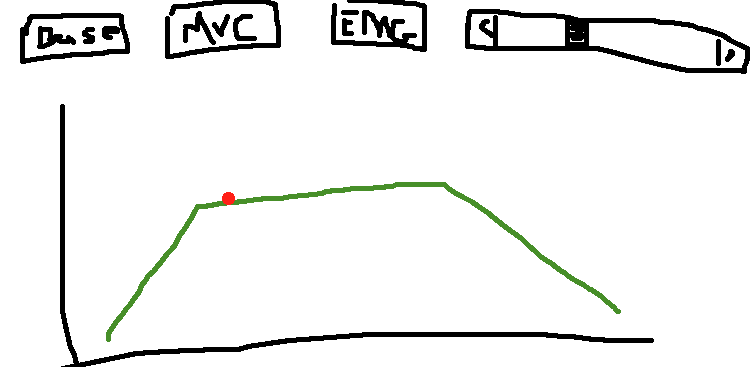
\includegraphics[width=0.5\textwidth]{figures/pMethods/GUIplot}
	\caption{The implemented GUI in MatLab, during data acquisition. \textbf{new picture}}
	\label{fig:GUIplot}
\end{figure}
